\chapter{Background}
\label{background}

%2.1-open neuro science
\cite{abrams2021standards}
% 2.1.1 data and tool sharing in neuroscience

% the platfroms that share tools and pipelines , (the infrustructure)  an overview of CONP as well

In this chapter, in section one we explain what Open Science is, FAIR principles~\cite{FAIR_Principles} which are defined for open science, and how open science can be helpful for researchers and scientists. We will then explain that open science is highly noticeable in neuroscience in section two and will write about some of the existing data and tool sharing platforms which attempt to guarantee FAIR principles~\cite{wilkinson2016fair}. In section three we will explain the recommender systems and the two main strategies.

% , there is no infrastructure which helps researchers in creating relevant analysis from these resources which led us to generate a recommender system for scientific pipelines and datasets.

% we explained the existing open neuroscience platforms, that they apply FAIR principles for the datasets, resources and analysis tools integrated on them. Therefore the user of these platforms has access to the previous analysis stored on the platforms and can run tool or pipeline on a dataset. However, the users are assisted until this phase, and there is no reliable system to help them select the appropriate pipeline and dataset for their analysis. In our project, we investigate the feasibility creating a recommender system to recommend pipelines and datasets based on the records from previous executions. 



\section{Open Science}

Open science is a collection of actions designed to make scientific processes more transparent and results more accessible. Its goal is to build a more replicable and robust science~\cite{spellman_gilbert_corker_2017}. Open science means that all steps in scientific research (including publications, data, physical samples, and software) should be publicly accessible to all levels of an inquiring society, amateur or professional~\cite{woelfle2011open}. In 2016 ‘FAIR Guiding Principles for scientific data management and stewardship’ were published and intended to provide guidelines to improve the Findability, Accessibility, Interoperability, and Reusability of digital assets with the objective of promoting open science. Importantly, these principles apply not only to ‘data’ in the conventional sense, but also to the algorithms, tools, and workflows that led to that data. All scholarly digital research objects (from data to analytical pipelines) benefit from application of these principles, since all components of the research process must be available to ensure transparency, reproducibility, and reusability.

\subsection*{Findability}
Finding the data is the first step of reusing them so metadata and data should be easy to find for both humans and computers, to achieve that, it is essential for the metadata to be machine-readable for automatic discovery of datasets and services.
Findability includes four principles:
\subsubsection*\quad \textbf{F1. (Meta)data are assigned a globally unique and persistent identifier}
Principle F1 is arguably the most important because it will be hard to achieve other aspects of FAIR without globally unique and persistent identifiers. Globally unique and persistent identifiers remove ambiguity in the meaning of your published data by assigning a unique identifier to every element of metadata and every concept/measurement in your dataset. In this context, identifiers consist of an internet link (e.g., a URL that resolves to a web page that defines the concept such as a particular human protein). Many data repositories will automatically generate globally unique and persistent identifiers to deposited datasets. Identifiers are essential to the human-machine interoperation that is key to the vision of Open Science. In addition, identifiers will help others to properly cite your work when reusing your data.

\subsubsection*\quad \textbf{F2. Data are described with rich metadata}
In creating FAIR digital resources, metadata can (and should) be generous and extensive, including descriptive information about the context, quality and condition, or characteristics of the data. Rich metadata allows a computer to automatically accomplish routine and tedious sorting and prioritising tasks that currently demand a lot of attention from researchers. The rationale behind this principle is that someone should be able to find data based on the information provided by their metadata, even without the data’s identifier. As such, compliance with F2 helps people to locate your data, and increase re-use and citations. Rich metadata implies that you should not presume that you know who will want to use your data, or for what purpose. 

\subsubsection*\quad \textbf{F3. Metadata clearly and explicitly include the identifier of the data they describe}
This is a simple and obvious principle, but of critical importance to FAIR. The metadata and the dataset are  usually separate files. The association between a metadata file and the dataset should be made explicit by mentioning a dataset’s globally unique and persistent identifier in the metadata. As stated in F1, many data repositories will generate globally unique and persistent identifiers for deposited datasets that can be used for this purpose.

\subsubsection*\quad \textbf*{F4. (Meta)data are registered or indexed in a searchable resource}
Identifiers and rich metadata descriptions alone will not ensure ‘findability’ on the internet. Sometimes, good data resources may go unused simply because no one knows they exist. If the availability of a digital resource such as a dataset, service or repository is not known, then nobody (and no machine) can discover it. There are many ways in which digital resources can be made discoverable, including indexing. For example, Google sends out spiders that ‘read’ web pages and automatically index them, so they then become findable in the Google search box. This is great for most ordinary searchers, but for scholarly research data, we need to be more explicit about indexing. Principles F1-F3 will provide the core elements for fine-grained indexing by some current repositories and future services.

\subsection*{Accessibility}

Once the user finds the required data, they need to know how can the data be accessed, possibly including authentication and authorisation.

\subsubsection*{A1. (Meta)data are retrievable by their identifier using a standardised communications protocol}
Most users of the internet retrieve data by ‘clicking on a link’. This is a high-level interface to a low-level protocol called tcp~\cite{forouzan2002tcp}, that the computer executes to load data in the user’s web browser. (Note that http(s) or ftp, which form the backbone of modern internet, are built on tcp, and make requesting and providing digital resources substantially easier than other communication protocols.) Principle A1 states that FAIR data retrieval should be mediated without specialised or proprietary tools or communication methods. This principle focuses on how data and metadata can be retrieved from their identifiers
\subsubsection*\quad \textbf{A1.1.The protocol is open, free, and universally implementable}

To maximise data reuse, the protocol should be free (no-cost) and open (-sourced) and thus globally implementable to facilitate data retrieval. Anyone with a computer and an internet connection can access at least the metadata. Hence, this criterion will impact your choice of the repository where you will share your data.

\subsubsection*\quad \textbf{A1.2. The protocol allows for an authentication and authorisation procedure, where necessary}

The ‘A’ in FAIR does not necessarily mean ‘open’ or ‘free’. Rather, it implies that one should provide the exact conditions under which the data are accessible. Hence, even heavily protected and private data can be FAIR. Ideally, accessibility is specified in such a way that a machine can automatically understand the requirements, and then either automatically execute the requirements or alert the user to the requirements. It often makes sense to request users to create a user account for a repository. This allows to authenticate the owner (or contributor) of each dataset, and to potentially set user-specific rights. Hence, this criterion will also affect your choice of the repository where you will share your data.


\subsubsection*{A2. Metadata are accessible, even when the data are no longer available}

Datasets tend to degrade or disappear over time because there is a cost to maintaining an online presence for data resources. When this happens, links become invalid and users waste time hunting for data that might no longer be there. Storing the metadata generally is much easier and cheaper. Hence, principle A2 states that metadata should persist even when the data are no longer sustained. A2 is related to the registration and indexing issues described in F4. 


\subsection*{Interoperability}
The data usually need to be integrated with other data. In addition, the data need to interoperate with applications or workflows for analysis, storage, and processing.


\subsubsection*{I1. (Meta)data use a formal, accessible, shared, and broadly applicable language for knowledge representation}
Humans should be able to exchange and interpret each other’s data, however, this also applies to computers, meaning that the data should be readable for machines without the need for specialised or ad-hoc algorithms, translators, or mappings. Interoperability typically means that each computer system at least has knowledge of the other system’s data exchange formats. For this to happen and to ensure automatic findability and interoperability of datasets, it is critical to use (1) commonly used controlled vocabularies, anthologies, thesauri (having resolvable globally unique and persistent identifiers, see F1) and (2) a good data model (a well-defined framework to describe and structure (meta)data).

\subsubsection*{I2. (Meta)data use vocabularies that follow FAIR principles}
The controlled vocabulary used to describe datasets needs to be documented and resolvable using globally unique and persistent identifiers. This documentation needs to be easily findable and accessible by anyone who uses the dataset.

\subsubsection*{I3. (Meta)data include qualified references to other (meta)data}
A qualified reference is a cross-reference that explains its intent. For example, X is regulator of Y is a much more qualified reference than X is associated with Y, or X see also Y. The goal therefore is to create as many meaningful links as possible between (meta)data resources to enrich the contextual knowledge about the data, balanced against the time/energy involved in making a good data model. To be more concrete, you should specify if one dataset builds on another data set, if additional datasets are needed to complete the data, or if complementary information is stored in a different dataset. In particular, the scientific links between the datasets need to be described. Furthermore, all datasets need to be properly cited (i.e., including their globally unique and persistent identifiers).






\subsection*{Reusability}
The ultimate goal of FAIR is to optimise the reuse of data. To achieve this, metadata and data should be well-described so that they can be replicated and/or combined in different settings.





\subsubsection*{R1. (Meta)data are richly described with a plurality of accurate and relevant attributes}
It will be much easier to find and reuse data if there are many labels are attached to the data. Principle R1 is related to F2, but R1 focuses on the ability of a user (machine or human) to decide if the data is actually USEFUL in a particular context. To make this decision, the data publisher should provide not just metadata that allows discovery, but also metadata that richly describes the context under which the data was generated. This may include the experimental protocols, the manufacturer and brand of the machine or sensor that created the data, the species used, the drug regime, etc. Moreover, R1 states that the data publisher should not attempt to predict the data consumer’s identity and needs. We chose the term ‘plurality’ to indicate that the metadata author should be as generous as possible in providing metadata, even including information that may seem irrelevant.

\subsubsection*\quad \textbf{R1.1. (Meta)data are released with a clear and accessible data usage license}

Under ‘I’, we covered elements of technical interoperability. R1.1 is about legal interoperability. What usage rights do you attach to your data? This should be described clearly. Ambiguity could severely limit the reuse of your data by organisations that struggle to comply with licensing restrictions. Clarity of licensing status will become more important with automated searches involving more licensing considerations. The conditions under which the data can be used should be clear to machines and humans.


\subsubsection*\quad \textbf{R1.2. (Meta)data are associated with detailed provenance}

For others to reuse your data, they should know where the data came from (i.e., clear story of origin/history, see R1), who to cite and/or how you wish to be acknowledged. Include a description of the workflow that led to your data: Who generated or collected it? How has it been processed? Has it been published before? Does it contain data from someone else that you may have transformed or completed? Ideally, this workflow is described in a machine-readable format.


\subsubsection*\quad \textbf{R1.3. (Meta)data meet domain-relevant community standards}

It is easier to reuse data sets if they are similar: same type of data, data organised in a standardised way, well-established and sustainable file formats, documentation (metadata) following a common template and using common vocabulary. If community standards or best practices for data archiving and sharing exist, they should be followed. For instance, many communities have minimal information standards (e.g., MIAME, MIAPE). FAIR data should at least meet those standards.  Other community standards may be less formal, but nevertheless, publishing (meta)data in a manner that increases its use(ability) for the community is the primary objective of FAIRness. In some situations, a submitter may have valid and specified reasons to divert from the standard good practice for the type of data to be submitted. This should be addressed in the metadata. Note that quality issues are not addressed by the FAIR principles. The data’s reliability lies in the eye of the beholder and depends on the intended application.



\section{Open neuroscience}
In the world of neuroscience a lot of attempts have been
 made to simplify reproducible research, specifically in neuroimaging, and functional Magnetic Resonance Imaging (fMRI)\cite{Schottner_2020}. Also it is important for such platforms to satisfy FAIR principles. Among the existing platfroms for open neuroscience, we introduce OpenNuero, NeuroImaging Tools \& Resources Collaboratory (NITRIC) and Canadian Open Neuroscience Platform (CONP).


\subsection{OpenNeuro}
\href{https://openneuro.org}{OpenNeuro}, formerly known as OpenfMRI\cite{poldrack2017openfmri}, is a free online platform for storing, sharing and analysing of neuroimaging data~\cite{gorgolewski2017openneuro}. Researchers can upload their own data to share it with others and download others shared data, also they can run analysis pipelines on the data. 

\subsubsection{Uploading and sharing the data}
 OpenNeuro only accepts BIDS~\cite{gorgolewski2016brain} compatible datasets,(MRI, MEG, EEG, iEEG, ECoG, ASL, and PET data), and all datasets will by validated to be BIDS compatible before being uploaded. In OpenNeuro, when uploading data, users can specify if their data will be accessible publicly or not, however, the user agrees that the uploaded data on will be publicly accessible after 18 months. After uploading the data on OpenNeuro, the users are able to change the dataset, change metadata, apply versioning on the dataset or make copies of the dataset to guarantee the reputability of analysis. 
 
 The users can share their uploaded data with other colleagues or researchers and specify the level of access ranging from viewing to administration 

\subsubsection{Running analysis on the data }
The most exiting feature of OpenNeuro is that the users are able to run different analysis on the data and share the results of that. The user can select one of the containerized analysis pipelines among all available BIDS Apps to apply on the dataset. The only applicable tools are BIDS Apps~\cite{gorgolewski2017bids} since, as mentioned above, OpenNeuro accept only BIDS compatible dataset. After selecting a BIDS App, the user can set parameters and specify if the analysis should run on the whole dataset or on specific subject or sessions. Then the user can download all the generated results, use them for higher level costume analysis and the will have access to all logs for the executed analysis and will be able to debug the process if it has failed.


\subsection{NeuroImaging Tools and Resources Collaboratory (NITRIC)} 
The Neuroimaging Informatics Tools and Resources Collaboratory
(\href{www.nitrc.org}{NITRIC}) provides a triad of services include a Resources Registry (NITRIC-R), Image Repository (NITRIC-IR) and a cloud Computational Environment (NITRIC-CE) to meet the needs of the neuroimaging researchers\cite{kennedy2016nitrc,howToCiteNITRIC_website}\MM{how to cite nitric website as they mentioned?}.



% NITRC provides image-sharing functionality through both the NITRC Resource
% Registry (NITRC-R), where bulk data files can be released through the file release system (FRS), and the NITRC
% Image Repository (NITRC-IR), a XNAT-based image data management system. Currently hosting 14 projects,
% 6845 subjects, and 8285 MRI imaging sessions, NITRC-IR provides a large array of structural, diffusion and resting
% state MRI data.
\subsubsection{NITRIC-R}

Resources, in this case, are broadly defined to include software, hardware, data,
websites, community organizations, etc. NITRC-R gives researchers greater and more efficient access to the tools and resources they need, better categorizing and organizing existing tools and resources, facilitating interactions between researchers and developers, and promoting better use through enhanced documentation and tutorials, forums, and updates. 

Each NITRC project has a homepage that describes the resources, provides
a standard set of resource characteristics (i.e. keywords, license,
dependencies, etc.), and provides a standard set of links for the resources
(i.e. download, documentation, support, etc.). Each resource page is
maintained by the resource administrator, who is responsible for
keeping it up to date. For every
project, resource administrators are also free to enable/disable any
functionality and redirect any content to other sources, as pertinent to
the resource developers' needs. Visitors to the NITRC site can search
for resources based on keywords, free text and specific capabilities in
order to find relevant resources. Currently, there are more that 1200 registered tools and 43000 registered users in NITRIC-R. 

\subsubsection{NITRIC-IR}

NITRC Image Repository offers a cloud-based federated neuroimaging data storage system for resource sharing of neuroimaging data in DlCOM and NIfTI formats. Currently it includes thousands of subjects and imaging sessions searchable across over a dozen projects to promote re-use and integration of valuable NIH-funded data.

The NITRC-IR is built on XNAT~\cite{marcus2007extensible} and provides sharing infrastructure for images and related data that can be closely integrated with the NITRC-R resources in order to better, support, promote, and manage data sharing functions for NITRC-hosted projects.
NITRC-R projects can be associated with NITRC-IR (XNAT) ‘projects’ and these can be interlinked. 
% From the search results you may select and download images. NITRC's Image Repository leverages XNAT software: Extensible Neuroimaging Archive Toolkit. 


\subsubsection{NITRIC-CE}

The NITRC Computational Environment is a freely downloadable, virtual computing cloud-based platform built upon a NeuroDebian operating system. NITRC-CE preinstalls popular neuroimaging tools such as AFNI, ANTS, FreeSurfer, FSL, C-PAC, and MRIcron (for the complete list of tools click \href{https://www.nitrc.org/plugins/mwiki/index.php/nitrc:User_Guide_-_NITRC-CE_Installed_Packages}{here}) into a standardized computational environment to help users analyze their data quickly and easily. This environment can be deployed in the cloud (using Amazon Web Services Elastic Compute Cloud (EC2) or the Microsoft Azure Cloud Computing Platform), or as a virtual machine for local use. To run analysis, NITRIC-CE can access data through NITRIC-IR, NITRIC-R, secure file transfer from outside sources, and file system mounting of AWS S3 resources.


% \subsubsection{Access and data sharing in NITRIC}
% Each NITRC project manages its own access policy. Data, in either
% NITRC-R or NITRC-IR can be completely open, not requiring any
% authentication; open to NITRC users; or open only to NITRC users who
% are registered with a specific project. 

% Data sharing within the NITRC-R is supported by the file release system (FRS) which provides support for release of packages, releases and files. Data sharing within the NITRC-IR is build around projects, subjects, sessions and assessors, and data access for the NITRC-CE is facilitated through access to NITRC-IR and NITRC-R.






\subsection{Canadian Open Neuroscience Platform (CONP)}

The Canadian Open Neuroscience Platform (CONP) provides an infrastructure for the promotion of open-science workflows and the sharing of neuroscience data. There are several open-source technologies integrated in CONP web portal to provide extensible distributed federation of datasets, unified search capabilities for data and software tools, the ability to run analyses either on High-Performance Computing (HPC) infrastructures or locally.


\begin{figure*}
    \centering
    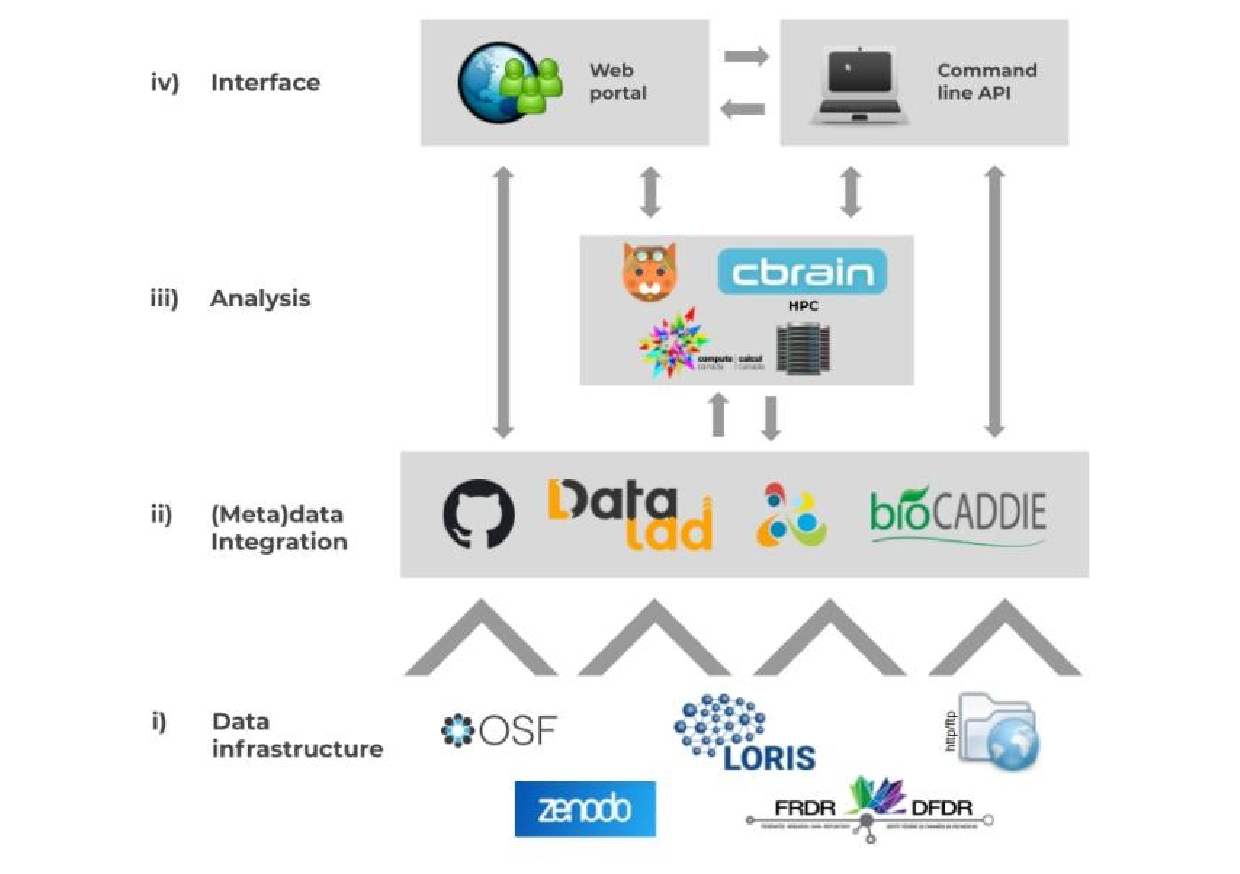
\includegraphics[width=\textwidth]{figures/CONP_figure.pdf}
    \caption{Architecture of the Canadian Open Neuroscience Platform. The platform is comprised of multiple tiers including:  i) independent data infrastructure; ii) Metadata integration across tools and datasets via standard models (Biocaddie DATS, Boutiques descriptors); iii) Data analysis on High-Performance Computing and; iv) Web and command-line interfaces. \cite{CONP}}
    \label{fig:CONP_figure}
\end{figure*}

Figure~\ref{fig:CONP_figure} illustrates the architecture of CONP and since we focused on the available datasets and pipelines in CONP in our project, we explain the levels of this structure in following. 

\subsubsection{Data infrastructure}
CONP employes different distributed data repositories with different infrastructures, access control requirements, APIs, and licensing such as domain-agnostic datastores (OSF, Zenodo, FRDR-DFDR), specific brain imaging repositories (LORIS, XNAT, Brain-CODE), and the commonly used HTTP and FTP web protocols. Also, CONP is extensible to any repository which allows access via programmatic web-compatible interfaces.

\subsubsection{Data integration}
In the (meta)data integration layer, CONP leverages DataLad~\cite{} as a backend, GitHub~\cite{} to host the metadata, and enables uniform data search queries based on the Data Tags Suite model~\cite{}. Datalad is responsible for integration between datasets, it is a software library for managing Git repositories referencing the data through storing metadata, file URLs and hashes of data managed by git-annex. Therefore, a DataLad dataset does not contain the data themselves, the actual datasets remain stored remotely.

The data themselves can be stored in any server implementing a protocol supported by git-annex, including HTTP, FTP, and many more. We used this flexibility to integrate data coming from three main types of sources. First, brain data archives such as the LORIS [13], XNAT [19], and Brain-CODE [20] platforms provide a complete neuroscience data management solution for data ingestion, quality control, visualization, access control, and querying. They are commonly used to support large-scale multi-site longitudinal studies with hundreds of participants. Second, multi-disciplinary research data archives such as Zenodo in Europe [4], the Open Science Framework in the USA [5], and the Federated Research Data Repository (FRDR) [21] in Canada, provide simple ways to share research data publicly through the web and to guarantee long-term archival, findability, and immutability of data objects through Digital Object Identifiers (DOIs). They are typically used for local studies or companion data to a publication. Third, simple internet hosts accessible through the HTTP or FTP protocol allow for flexible integration of any other data already available online. CONP also provides local data-hosting for users who do not have the resources to make use of these other options 



Also CONP uses the crawlers to automate the discovery of tools (on Zenodo) and datasets (on Zenodo and OSF) and the DataLad and GitHub integration workflows.

CircleCI~\cite{} continuously tests if datasets are available and if data are accessible by testing the download of a few files from the datasets. 


2.2.1 Integration of distributed datasets
The CONP adopts a decentralized architecture, to accommodate the various governance, ethical, and performance models required by data owners. For instance, some datasets may not easily be stored outside of the jurisdiction where they were acquired, while some institutions require local control of data storage, with some projects preferring to remain in control of access rules. This is all possible in CONP, as data can remain hosted anywhere on the internet.
Integration between datasets is provided by DataLad, a software library for managing Git repositories that reference data. In DataLad, datasets are described in a Git repository containing metadata, file URLs and hashes of data blobs managed by git-annex. Importantly, a DataLad dataset does not generally contain the data themselves, which remain stored remotely. DataLad datasets can also be nested to represent dataset aggregation.

The CONP dataset consists of a main DataLad dataset, its metadata -and possibly the data themselves when small- stored on GitHub and referenced in the main DataLad index. The use of GitHub enables a variety of features useful for open-source software development; including issue tracking, code reviews, pull requests, branch protection, and integration with various applications. Datasets are integrated as Git submodules of the main dataset, and may be hosted on GitHub or on any other platform including GitLab or even a simple web server. This has the added benefit of being able to point to a specific commit, allowing continued evolution of the remote subdataset while the CONP portal keeps a reference to the stable version of the root dataset. Any DataLad dataset can be integrated into CONP provided that it contains a README file and a Data Tags Suite (DATS [18]) model file describing it. In addition, a configuration script can be added to the root of the dataset, to perform any required initialization.








\subsubsection{Analysis and tools}
an analysis layer that allows for simple download of tools and easy use of High-Performance Computing (HPC) environments

\subsubsection{Interface}
an interface layer, which controls the interaction between these components and will be outlined further in the Results section


\section{recommender systems}
\subsection{Content based}
\subsection{collaborative filtering}


